\section{Implementation}
\label{sec:impl}

Beerculator's development can be split into three main categories, respectively described by {\sc subsections}~\ref{ssec:db}, \ref{ssec:java} and \ref{ssec:server}.

\subsection{Databases}
\label{ssec:db}

PostgreSQL was used for creating and managing the databases. There are three databases in the project, which are the following ones:

\begin{itemize}
\item drinks: contains all the predefined drinks that the user can select;
\item drink\_records: contains the drinks selected by the current user;
\item users: contains all informations about the different users.
\end{itemize}

The attributes of those databases, and also the way that they are linked to each other, are explained by {\sc figure}~\ref{fig:UMLdb}.

\begin{figure}[H]
\centering
   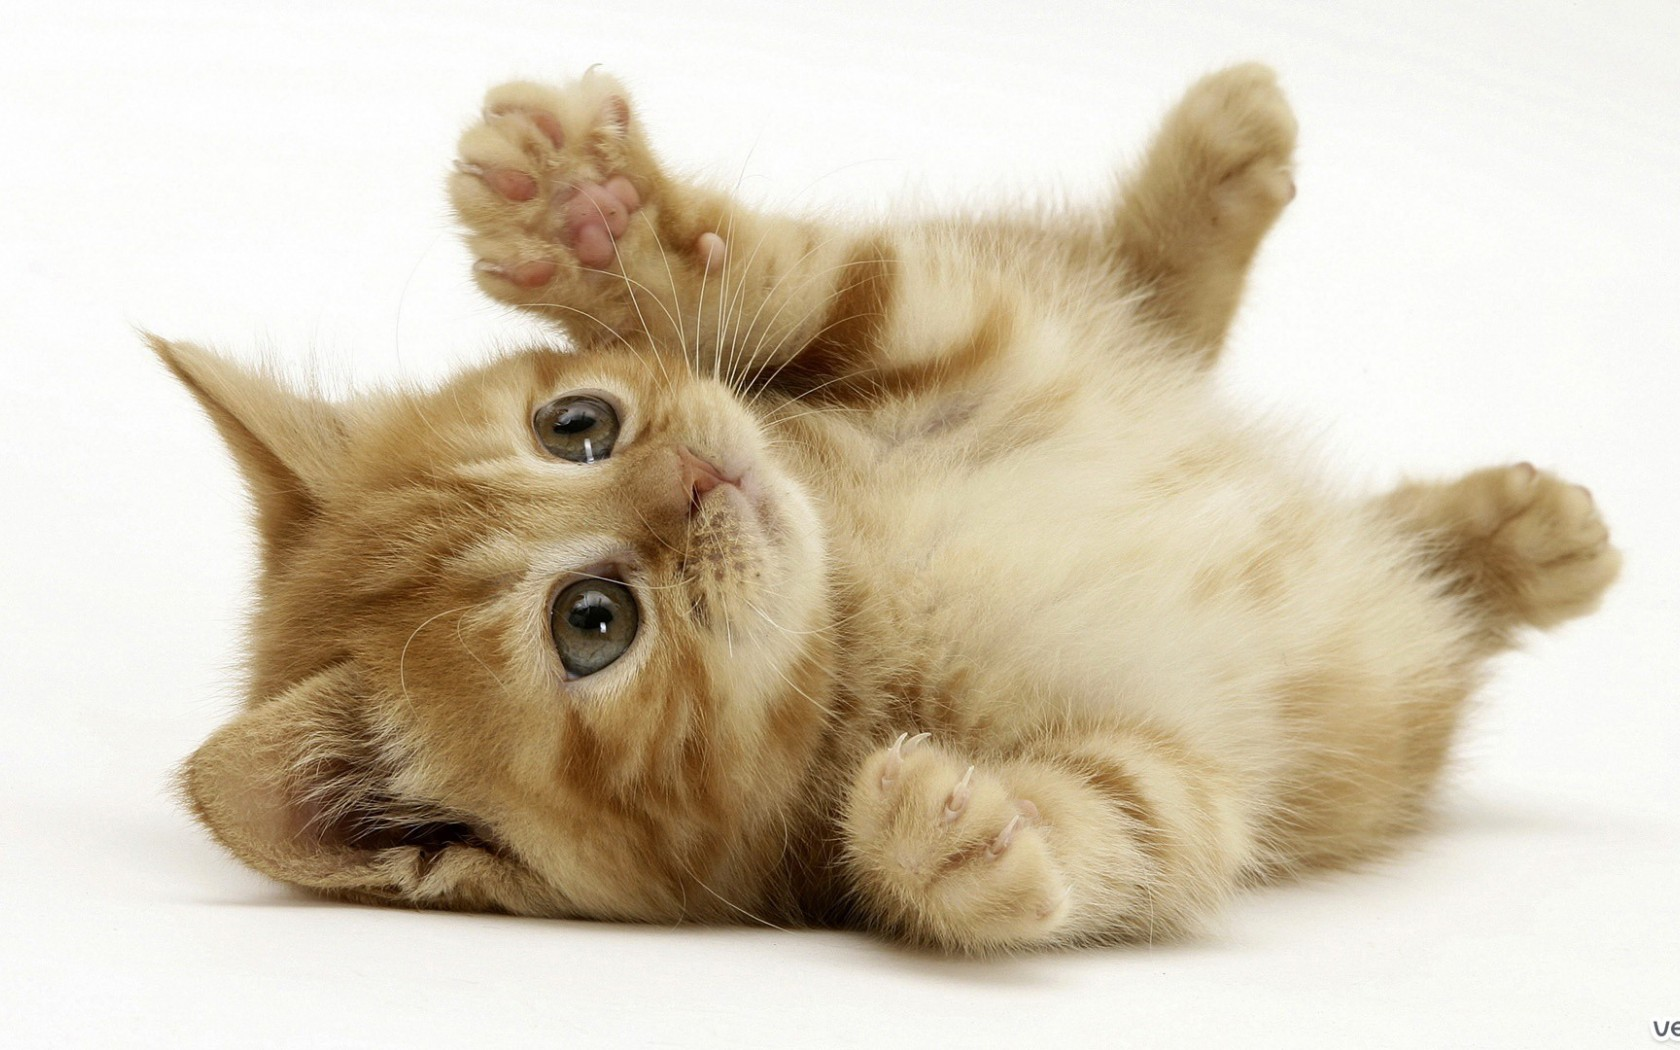
\includegraphics[scale=0.2]{./figures/uml_db.jpeg}
   \caption{UML diagrams for the databases}
   \label{fig:UMLdb}
\end{figure}

\subsection{Java}
\label{ssec:java}

Java was the heart of the project, as it was used to code the main program but also to perform all the calculations. The project consists in three main classes, Drink.java, DrinkRecord.java and User.java. Their respective UML representations are given by {\sc figures} \ref{fig:drinkJava}, \ref{fig:drinkRecordJava} and \ref{fig:userJava}.\\

It is interesting to notice that the calculation methods, calculateBAC() and hoursUntilSober(double), are implemented in User.java. They are based on the formulas previously introduced in {\sc section}~\ref{sec:spec}. 

\begin{figure}[H]
\centering
   \includegraphics{./figures/drink.png}
   \caption{Class Drink.java, its attributes and its methods}
   \label{fig:drinkJava}
\end{figure}

\begin{figure}[H]
\centering
   \includegraphics{./figures/drinkRecord.png}
   \caption{Class DrinkRecord.java, its attributes and its methods}
   \label{fig:drinkRecordJava}
\end{figure}

\begin{figure}[H]
\centering
   \includegraphics{./figures/user.png}
   \caption{Class User.java, its attributes and its methods}
   \label{fig:userJava}
\end{figure}

\subsection{Web content}
\label{ssec:server}